\section{LQG}
Рассмотрим систему: 
\begin{equation}
    \begin{cases}
        \dot{x} = Ax + Bu + f\\
        y = Cx + Du + \xi
    \end{cases}, \quad x_0 = \begin{bmatrix}1 & 1 & 1 & 1\end{bmatrix}^T
\end{equation} 
где
\begin{equation}
    \begin{array}{cccc}
        A = \begin{bmatrix}
            4 & -2 & 0 & 6 \\ 
            -2 & 4 & -6 & 0 \\
            0 & -6 & 4 & 2 \\
            6 & 0 & 2 & 4
        \end{bmatrix}, & 
        B = \begin{bmatrix}
            11 & 0 \\
            -1 & 0 \\
            7 & 0 \\ 
            9 & 0 \\
        \end{bmatrix}, & 
        C = \begin{bmatrix}
            1 & -1 & 1 & 1 \\
            1 & 3 & -1 & 3
        \end{bmatrix}, 
        D = \begin{bmatrix} 
            0 & 3 \\ 
            0 & 4
        \end{bmatrix}
    \end{array}
\end{equation}
\begin{equation}
    f(t) = \begin{bmatrix}3\sin(2t) & 2\cos(3t) & \sin(3t) & \cos(t)\end{bmatrix}^T \quad \xi(t) = \begin{bmatrix}3\cos(3t) & \sin(3t)\end{bmatrix}
\end{equation}

\subsection{Управляемость и наблюдаемость}
Для определения управляемости и наблюдаемость собственных чисел рассмотрим вещественную Жорданову форму системы:
\begin{equation}
    \begin{cases}
        \dot{\hat{x}} = P^{-1}AP\hat{x} + P^{-1}Bu \\
        \hat{y} = C\hat{x} + Du
    \end{cases}
\end{equation}
\begin{equation}
    \begin{array}{cccc}
        A_j = \begin{bmatrix}
            0.00  & 0.00  & 0.00  & 0.00 \\ 
            0.00  & -4.00  & 0.00  & 0.00 \\ 
            0.00  & 0.00  & 12.00  & 0.00 \\ 
            0.00  & 0.00  & 0.00  & 8.00 \\ 
            \end{bmatrix} &
        P = \begin{bmatrix}
            -1.00  & -1.00  & 1.00  & 1.00 \\ 
            1.00  & -1.00  & -1.00  & 1.00 \\ 
            1.00  & -1.00  & 1.00  & -1.00 \\ 
            1.00  & 1.00  & 1.00  & 1.00 \\ 
            \end{bmatrix}, \\
        B_j = \begin{bmatrix}
            1.00  & 0.00 \\ 
            -2.00  & 0.00 \\ 
            7.00  & 0.00 \\ 
            3.00  & 0.00 \\
            \end{bmatrix}, & 
        C_j = \begin{bmatrix}
            0.00  & 0.00  & 4.00  & 0.00 \\ 
            4.00  & 0.00  & 0.00  & 8.00 \\ 
        \end{bmatrix}
    \end{array}
\end{equation}

Можно сделать вывод, что система является полностью управляемой, а 
а собственное число $\lambda_2 = -4$ не является наблюдаемым. Соответственно, 
система не является полностью наблюдаемой, но, так как собственное число 
$\lambda_2$ располагается в левой полуплоскости, то система является обнаруживаемой. 

\subsection{Синтез LQG-регулятора}
Рассмотрим наблюдатель и регулятор 
\begin{equation}
    \dot{\hat{x}} = A\hat{x} + (B + LD)u + L(\hat{y} - y) \\ \quad u = K\hat{x}
\end{equation}
Будем использовать линейно-квадратичные уравнения для синтеза регулятора и LQE-наблюдателя. 
Порядок синтезы был рассмотрен в предыдущих задачах, поэтому сразу приведем матрицы 
весов $Q_K$, $R_K$ для синтеза регулятора и $Q_L$, $R_L$ для синтеза наблюдателя и 
полученные матрицы $K$ и $L$.
\begin{equation}
    Q_K = 30 \cdot I_{4\times4}, \quad R_K = 20
\end{equation}
\begin{equation}
    Q_L = 60 \cdot I_{4\times4}, \quad R_L = 2
\end{equation}
\begin{equation}
    \begin{array}{cc}
        K = \begin{bmatrix}
        5.99  & 19.14  & -20.41  & 4.82 \\ 
        0.00  & 0.00  & 0.00  & 0.00 \\
        \end{bmatrix} &
        L = \begin{bmatrix}
        -7.06  & -8.73 \\ 
        7.06  & -3.25 \\ 
        -7.06  & 8.73 \\ 
        -7.06  & -3.25 \\
        \end{bmatrix}
    \end{array}
\end{equation}
Проведем моделирование системы, замкнутой регулятором на основе вектора оценки 
состояния наблюдателем. Схема моделирования представлена на рисунке \ref{fig:lqg_scheme}.
\begin{figure}[ht!]
    \centering
    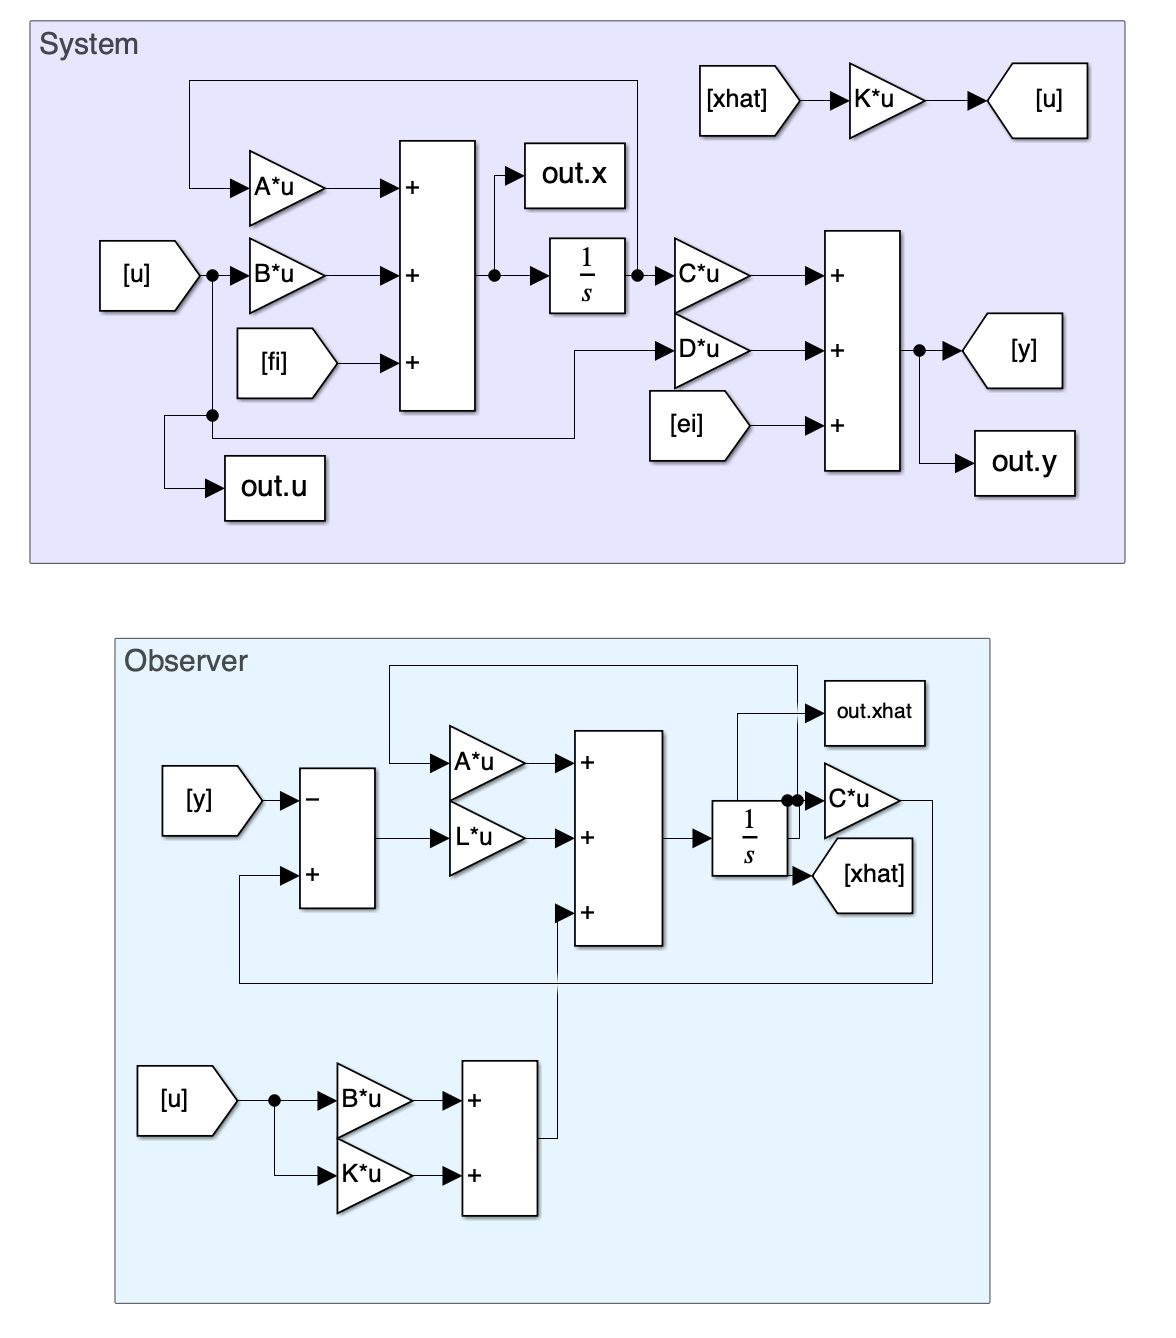
\includegraphics[width=0.8\textwidth]{media/lqg_cheme.png}
    \caption{Схема моделирования LQG-регулятора}
    \label{fig:lqg_scheme}
\end{figure}

График состояния системы и оценки состояния приведены на рисунке \ref{fig:lqg_state_cmp}, 
ошибка оценки состояния приведена на рисунке \ref{fig:lqg_state_err},
график управляющего воздействия на систему приведен на рисунке \ref{fig:lqg_u}, 
график выхода системы приведен на рисунке \ref{fig:lqg_y}.
\begin{figure}[ht!]
    \centering
    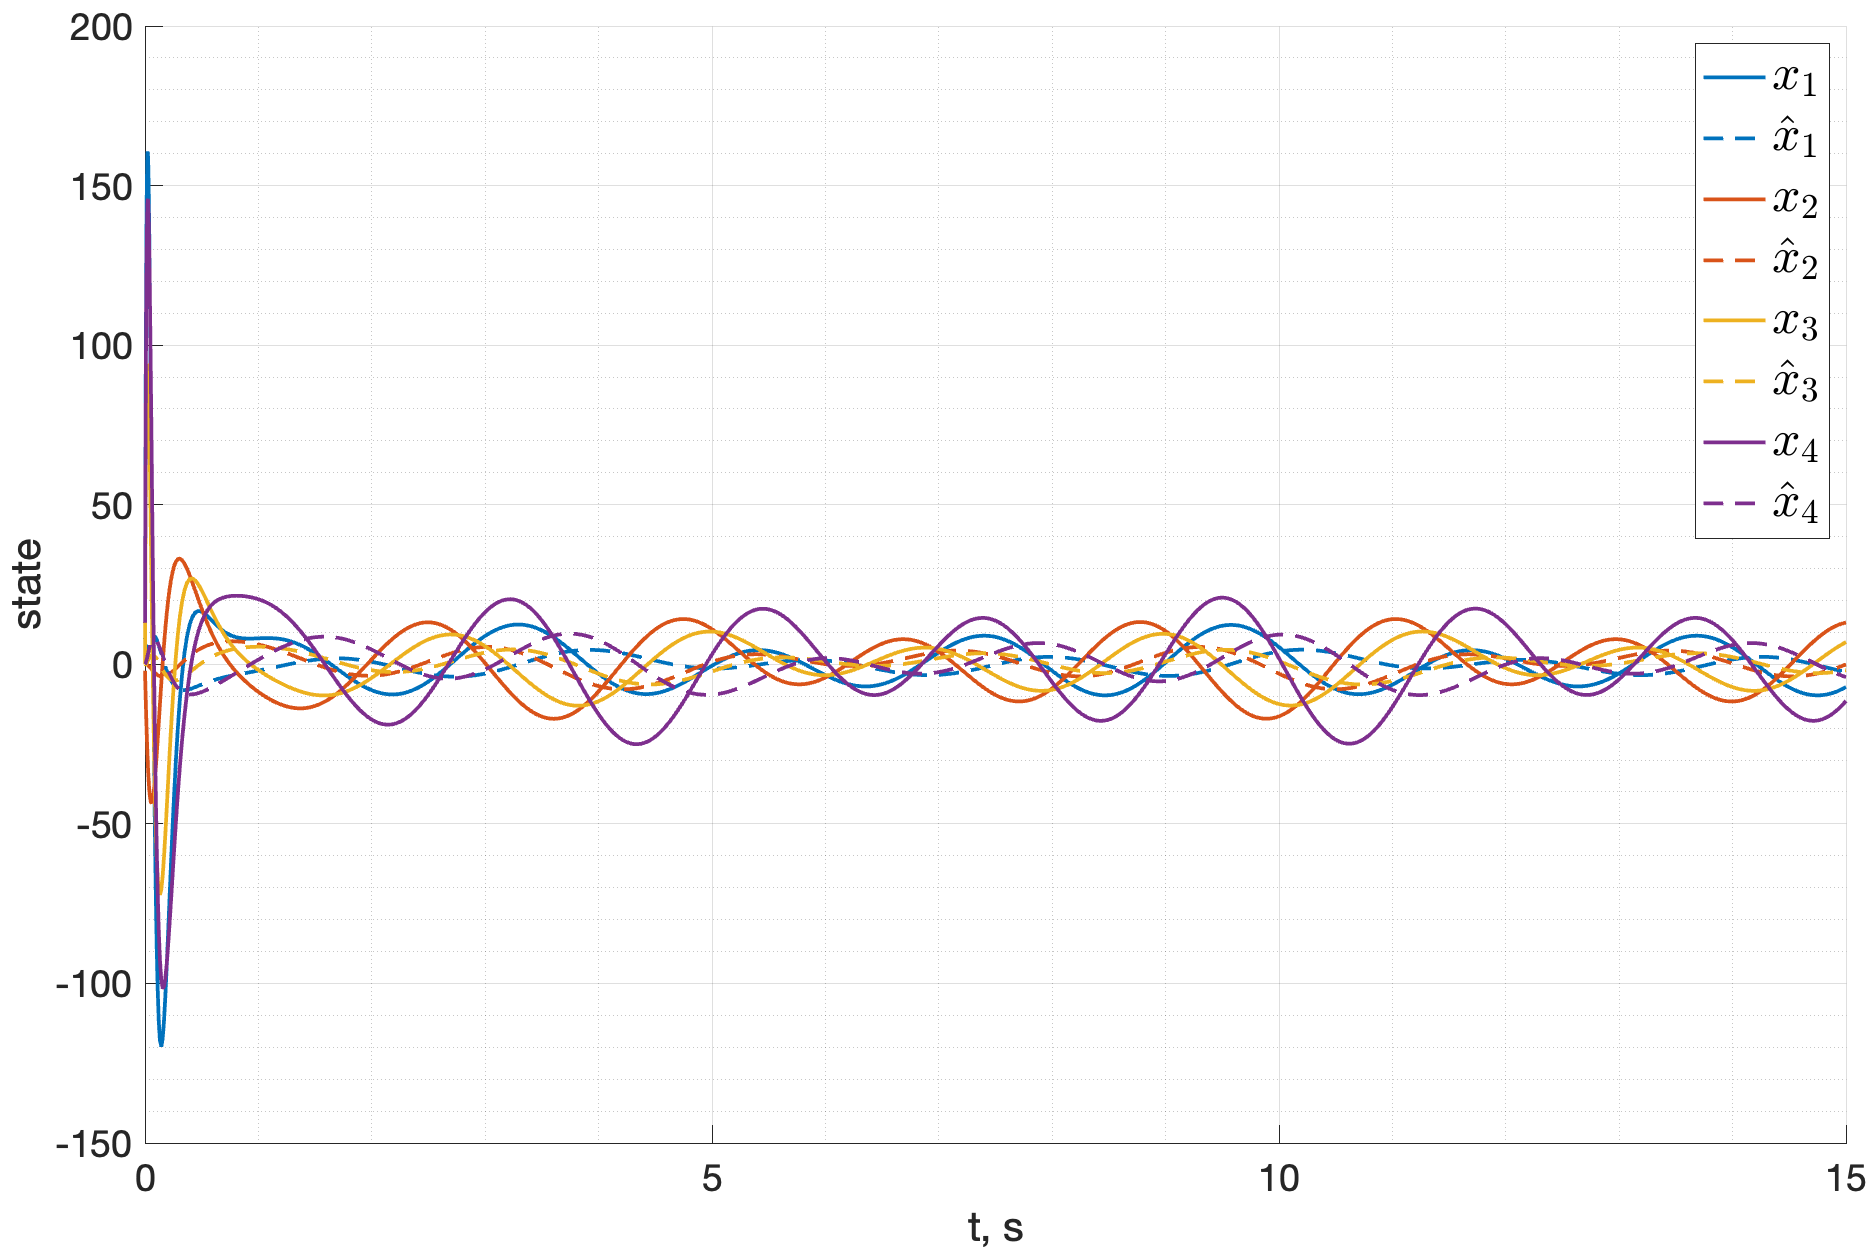
\includegraphics[width=\textwidth]{media/plots/lqr_task3/state_cmp_1.png}
    \caption{Сравнение состояния системы и оценки состояния}
    \label{fig:lqg_state_cmp}
\end{figure}
\begin{figure}[ht!]
    \centering
    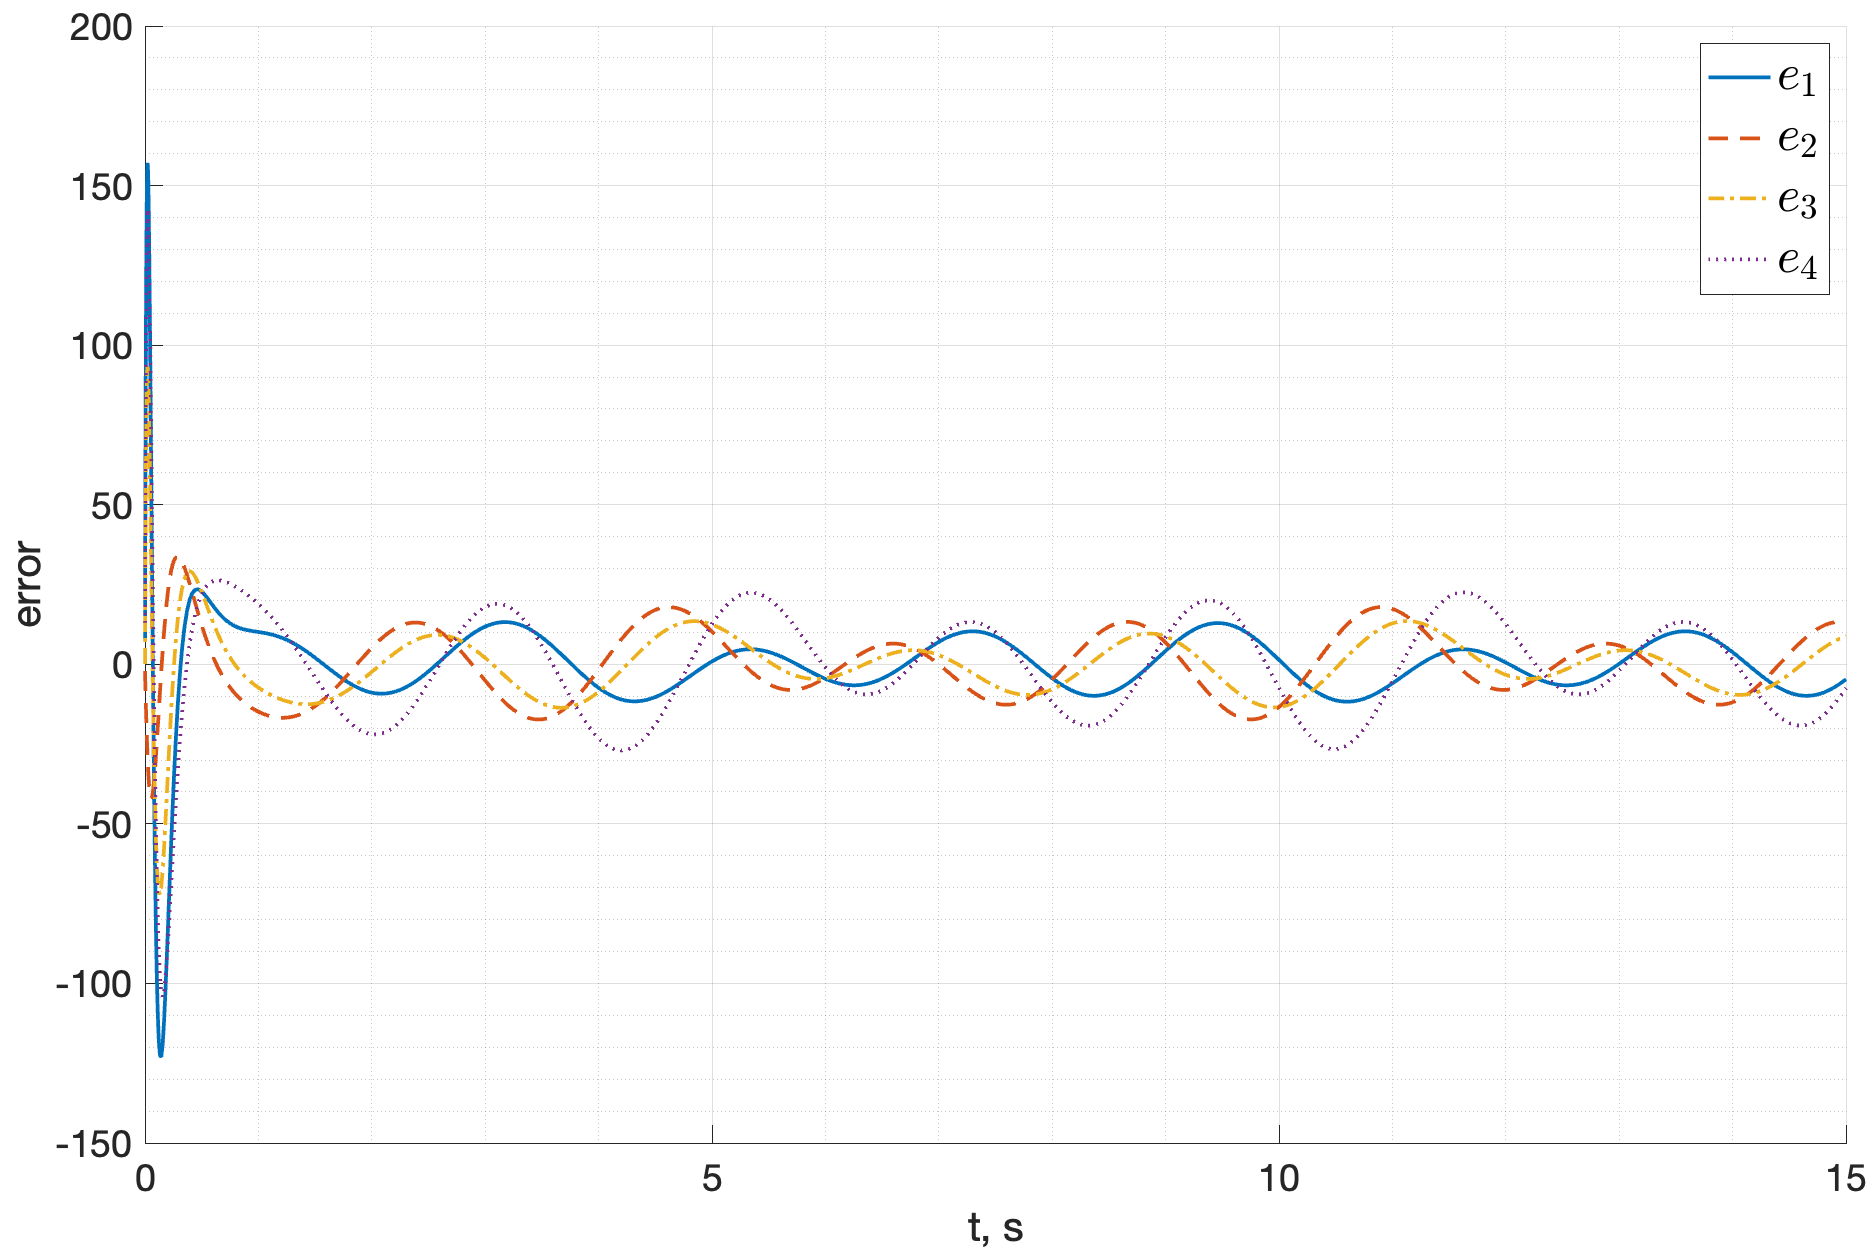
\includegraphics[width=\textwidth]{media/plots/lqr_task3/err_1.png}
    \caption{Ошибка оценки состояния}
    \label{fig:lqg_state_err}
\end{figure}
\begin{figure}[ht!]
    \centering
    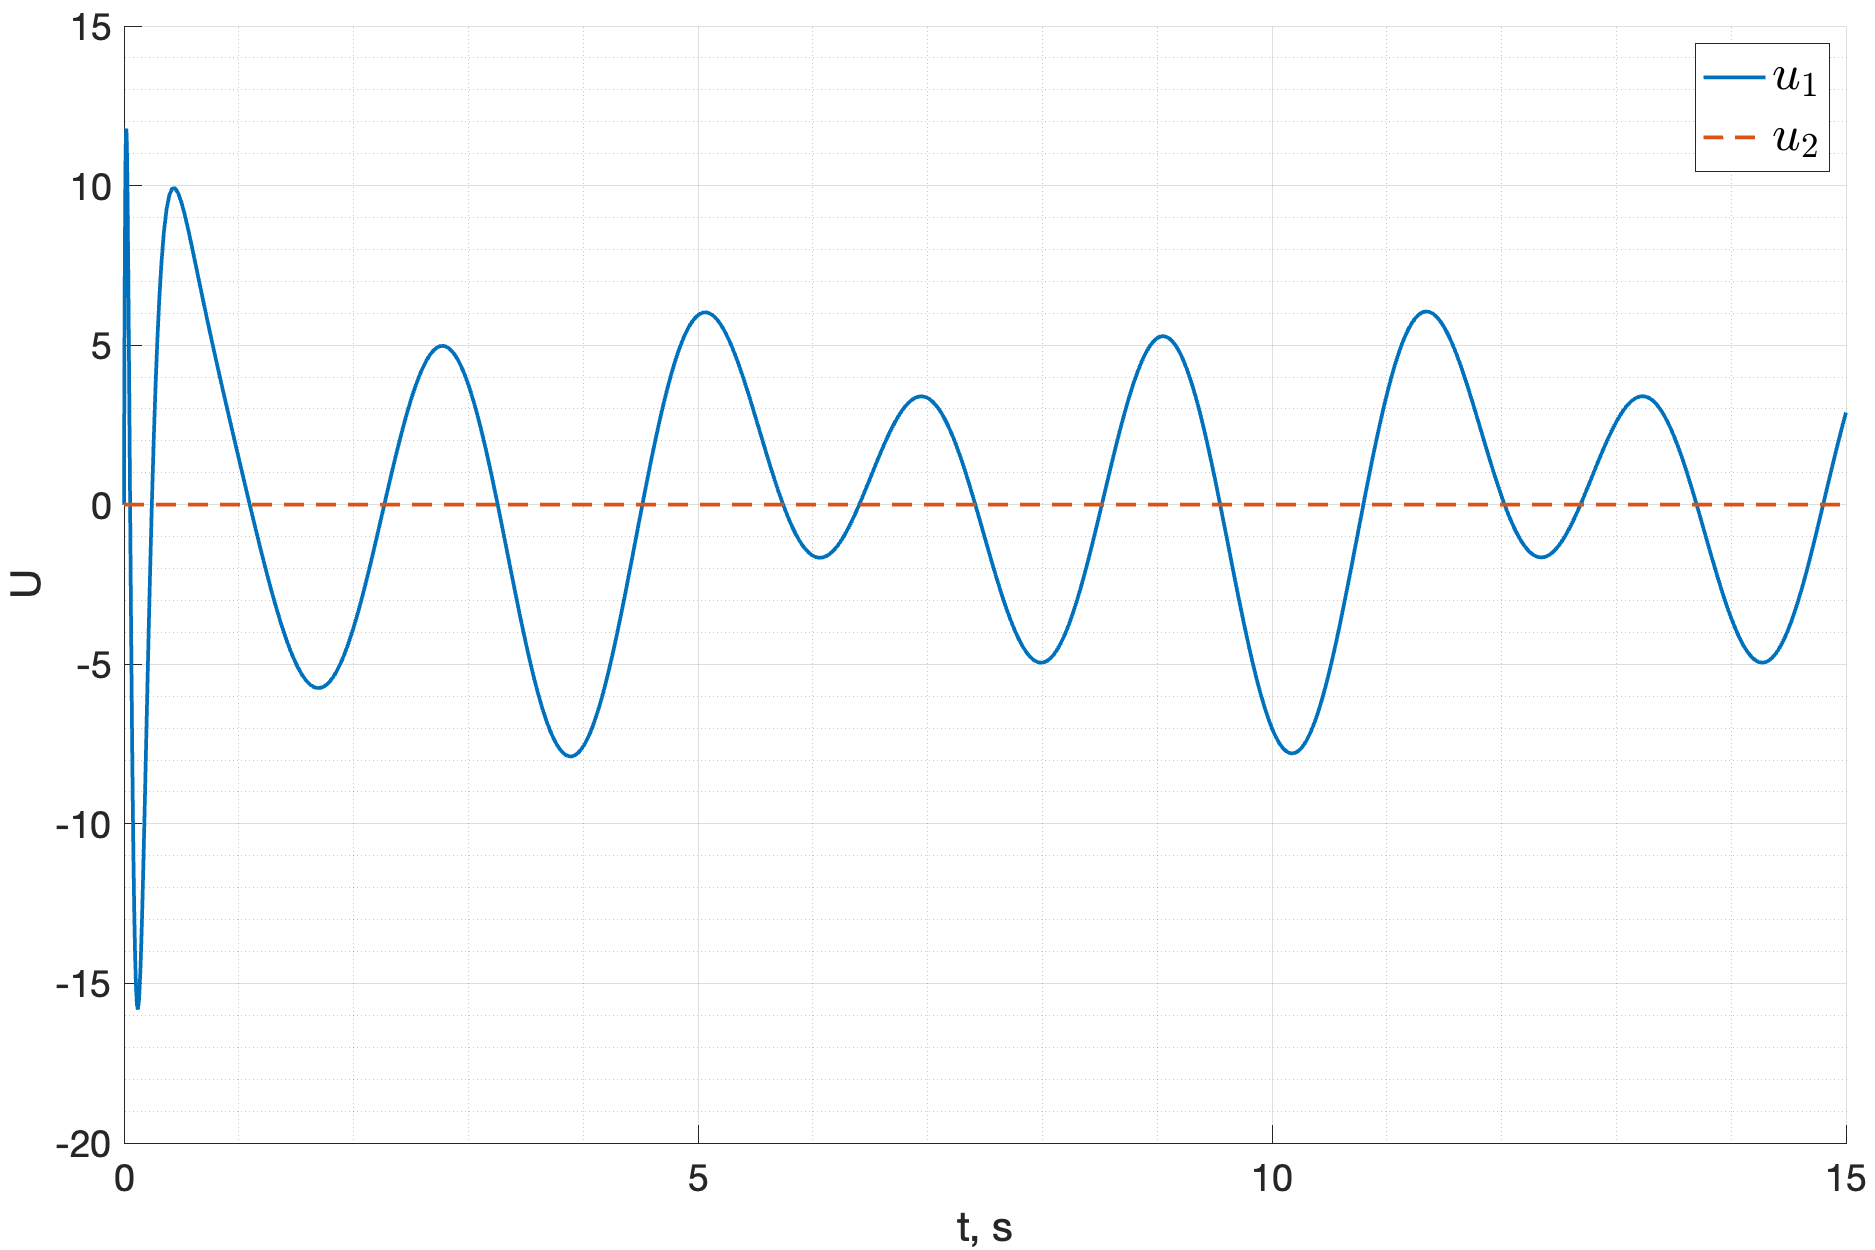
\includegraphics[width=\textwidth]{media/plots/lqr_task3/u_1.png}
    \caption{Управляющее воздействие на систему}
    \label{fig:lqg_u}
\end{figure}
\begin{figure}[ht!]
    \centering
    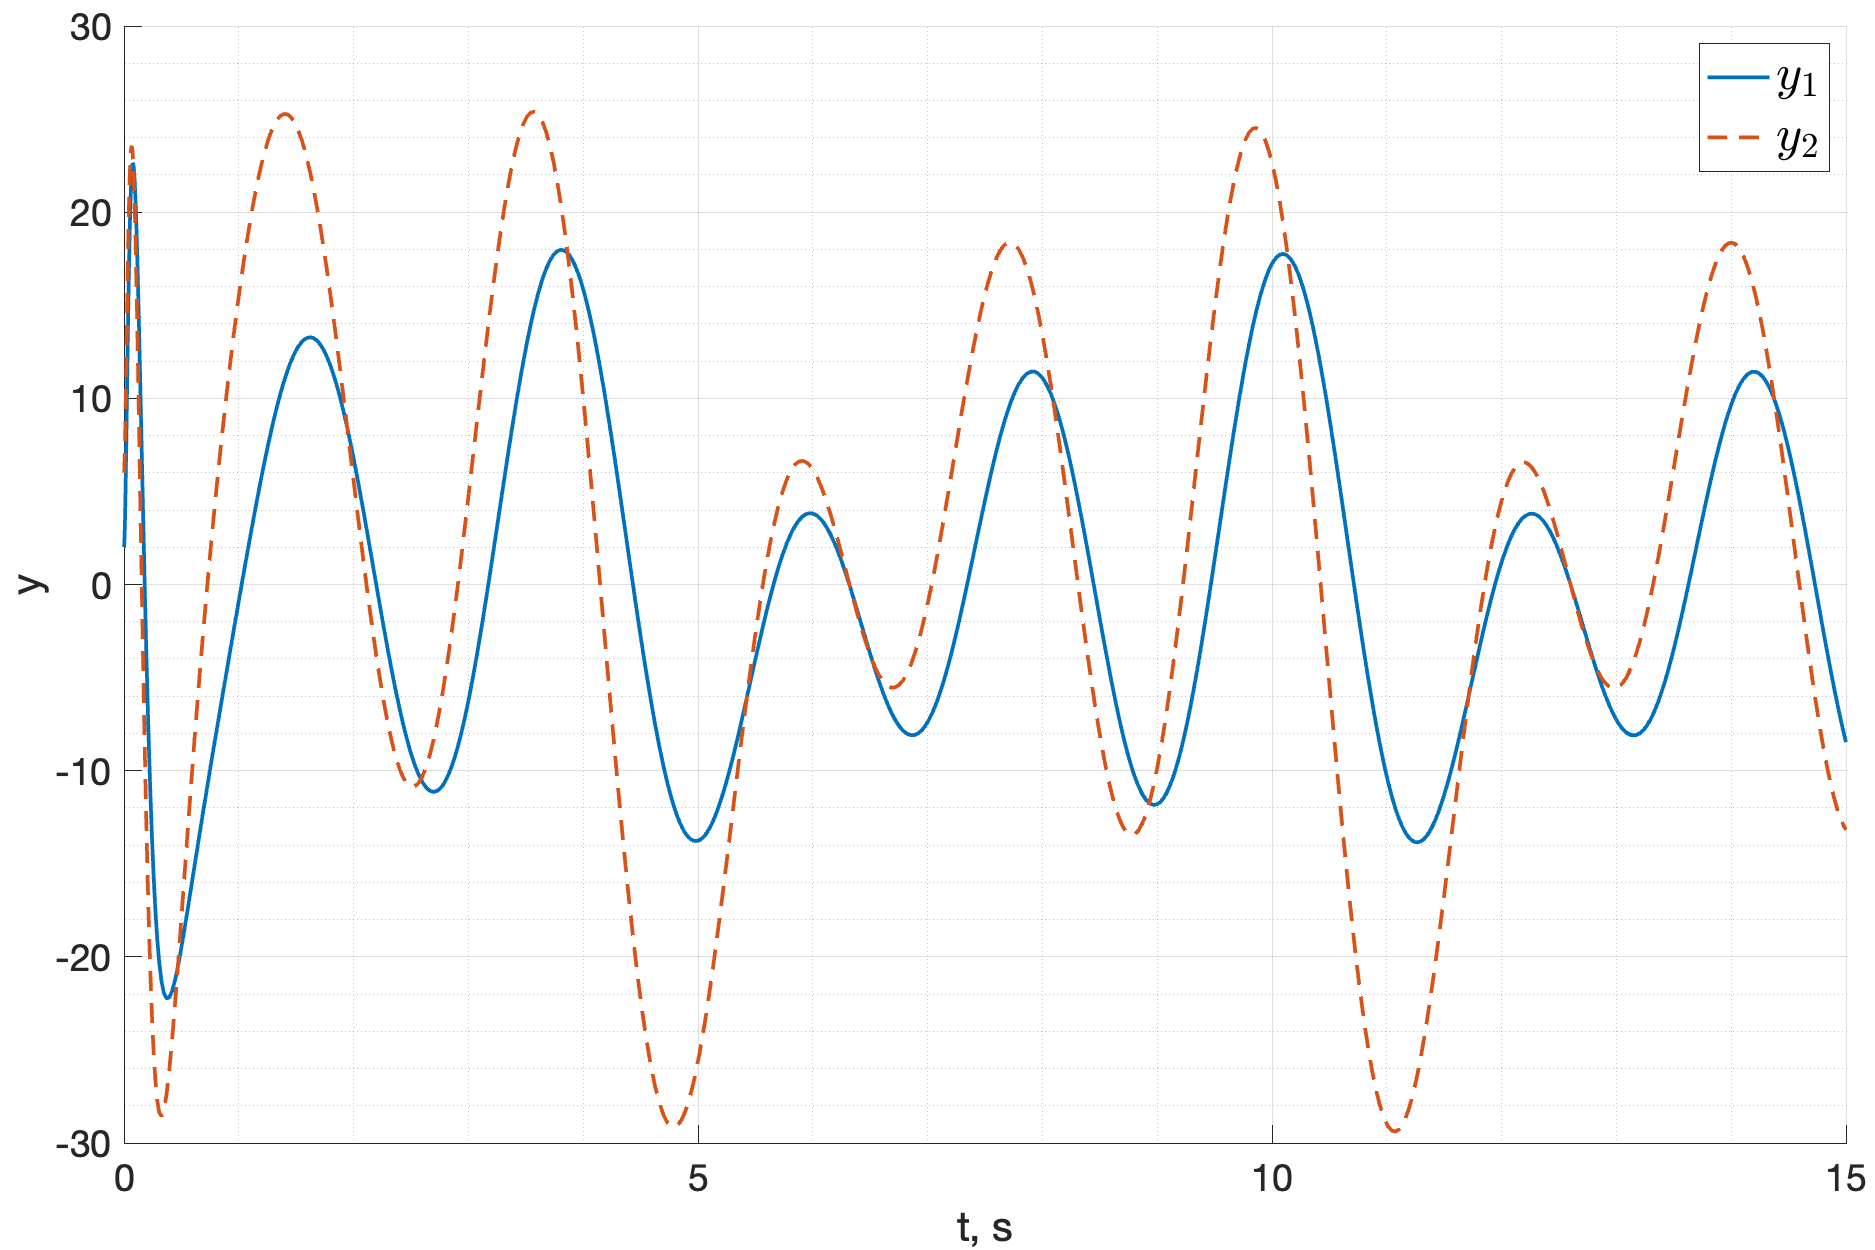
\includegraphics[width=\textwidth]{media/plots/lqr_task3/y_1.png}
    \caption{Выход системы}
    \label{fig:lqg_y}
\end{figure}
\FloatBarrier
\subsection{Выводы}
К сожалению, добиться полной стабилизации системы не удалось. Это связано с тем, 
что на систему действуют внешние возмущения, которые выводят ее из положения равновесия. 
К тому же, оценка состояния системы наблюдателем так же не является точной, в ошибке 
оценки состояния присутствуют колебания, которые также вызваны внешними возмущениями и 
шумом измерений, что также приводит к нестабильности системы. При этом, если посмотреть на 
собственные числа матрицы $A$, то можно заметить, что система не является устойчивой по Ляпунову
сама по себе, и должна \textit{разваливаться} без управления. Отсюда можно сделать вывод, что 
LQR регулятор не может полностью стабилизировать систему, но может значительно улучшить ее поведение. 